\documentclass{beamer}

%fonts related
\usepackage{helvet}
\renewcommand{\familydefault}{\sfdefault}
\usepackage{textcomp}

%spell related
\usepackage[spanish]{babel}
\usepackage[utf8]{inputenc}

%graphics related
\usepackage{adjustbox}
\usepackage{graphicx}
\usepackage{pstricks}

\usepackage{graphicx}

\title{\emph{FRAMEWORK} PARA LA AUTOMATIZACIÓN DE PRUEBAS DE INTERFAZ DE USUARIO
EN EL MÓDULO DE PRODUCTOS Y LISTAS DE PRECIOS DE \emph{SALESFORCE}}
\author{Carlos E. Caballero B.}
\date{\today}

\begin{document}

\begin{frame}
\titlepage
\end{frame}

\begin{frame}
\frametitle{Contenidos}
\tableofcontents
\end{frame}

\section{Introducción}

\subsection{Definición del problema}

\begin{frame}
\frametitle{Definición del problema}
\begin{columns}
\column{0.5\textwidth}
Siendo el módulo de productos y listas de precios componentes participes en la
funcionalidad provista por otros módulos de \emph{Salesforce}, un potencial
error en este podría tener un efecto en cascada con el potencial de afectar el
servicio completo.
\column{0.5\textwidth}
\emph{Salesforce} sigue un política de actualizaciones muy continua, pudiendo
existir hasta tres versiones por año, lo que sin una automatización correcta
de las pruebas de interfaz de usuario, implicaría un enorme gasto de recursos
para la compañía.
\end{columns}
\end{frame}

\begin{frame}
\frametitle{Definición del problema}
\emph{«Garantizar la calidad de los elementos que componen la interfaz de
usuario requiere de un proceso de evaluación continuada y eficiente, de forma
que los módulos evaluados y sus diferentes versiones contengan la menor
cantidad posible de errores.»}.
\end{frame}

\subsection{Objetivo general}

\begin{frame}
\frametitle{Objetivo general}
Implementar un \emph{framework} para la automatización de las pruebas de interfaz de
usuario en el módulo de Productos y Listas de Precios en \emph{Salesforce},
para garantizar un procedimiento continuo de evaluación y minimizar la cantidad
de errores que contiene el software.
\end{frame}

\subsection{Objetivos específicos}

\begin{frame}
\frametitle{Objetivos específicos}
\begin{itemize}
\item Formular los casos de prueba necesarios que los módulos de gestión de
    productos y listas de precios requieran para cubrir los atributos de calidad
    requeridos.
\item Diseñar e implementar los modelos y bibliotecas de funciones que
    conforman un \emph{framework} de automatización.
\item Automatizar los casos de prueba de las funciones que componen la interfaz
    de usuario del módulo de gestión de productos y listas de precios.
\end{itemize}
\end{frame}

\subsection{Justificación}

\begin{frame}
\frametitle{Justificación}
Con una estrategia de automatización implementada apropiadamente el tiempo de
evaluar las nuevas funcionalidades del sistema, además de la evaluación de las
funcionalidades antiguas será reducido drásticamente, consiguiendo mejorar la
cobertura de las pruebas.
\end{frame}

\section{Conceptos y definiciones}

\begin{frame}
\frametitle{Automatización}
Se conoce que en los siguientes escenarios es útil automatizar:
\begin{itemize}
    \item Los requerimientos no cambian frecuentemente.
    \item Se accede al aplicativo con múltiples y variados usuarios, roles y
        privilegios.
    \item El software es estable respecto a sus pruebas manuales.
    \item Se cuenta con el tiempo necesario para automatización en el proyecto.
    \item El proyecto sigue o debe seguir estándares estrictos.
    \item La complejidad del proyecto es elevada.
    \item El proyecto requiere constantes revisiones en algunas de sus
    características.
\end{itemize}
\end{frame}

\subsection{Automatización}

\begin{frame}
\frametitle{Automatización}
Los criterios a seguir son:
\begin{itemize}
    \item Identificar áreas dentro del software para automatizar.
    \item Elegir la herramienta adecuada para la automatización.
    \item Escribir las rutinas de prueba.
    \item Desarrollar el conjunto de casos de prueba.
    \item Ejecutar los casos de prueba.
    \item Generar los reportes de resultados.
    \item Encontrar los posibles errores o aspectos negativos.
\end{itemize}
\end{frame}

\begin{frame}
\frametitle{Automatización}
Los beneficios de la automatización son:
\begin{itemize}
    \item Incremento de la productividad.
    \item Ahorro de dinero, en el costo del proyecto.
    \item Aumento de la calidad del software.
    \item Reducción del tiempo de evaluación del software.
    \item Soporte para múltiples aplicativos del software.
    \item Aumento de la cobertura de las pruebas.
    \item Reducción del trabajo repetitivo.
    \item Mejora de la consistencia del producto.
\end{itemize}
\end{frame}

\begin{frame}
\frametitle{Automatización}
Los riesgos de la automatización son:
\begin{itemize}
    \item El costo de arranque de la automatización puede llegar a ser muy alto.
    \item Debe tenerse en cuenta que la automatización de las pruebas jamas
        podrá cubrir el 100\% de cobertura del software.
    \item No es conveniente automatizar una interfaz de usuario no establecida.
    \item Si la aplicación de usuario cambia constantemente, el costo de
        mantenimiento de las pruebas automatizadas será muy alto.
\end{itemize}
\end{frame}

\begin{frame}
\frametitle{Pirámide de automatización de pruebas.}
La pirámide de automatización de pruebas, es un concepto que fue introducido
por \emph{Cohn} en su articulo «\emph{Succeeding with Agile}», y describe como
equilibrar la automatización.
\begin{figure}
\centering
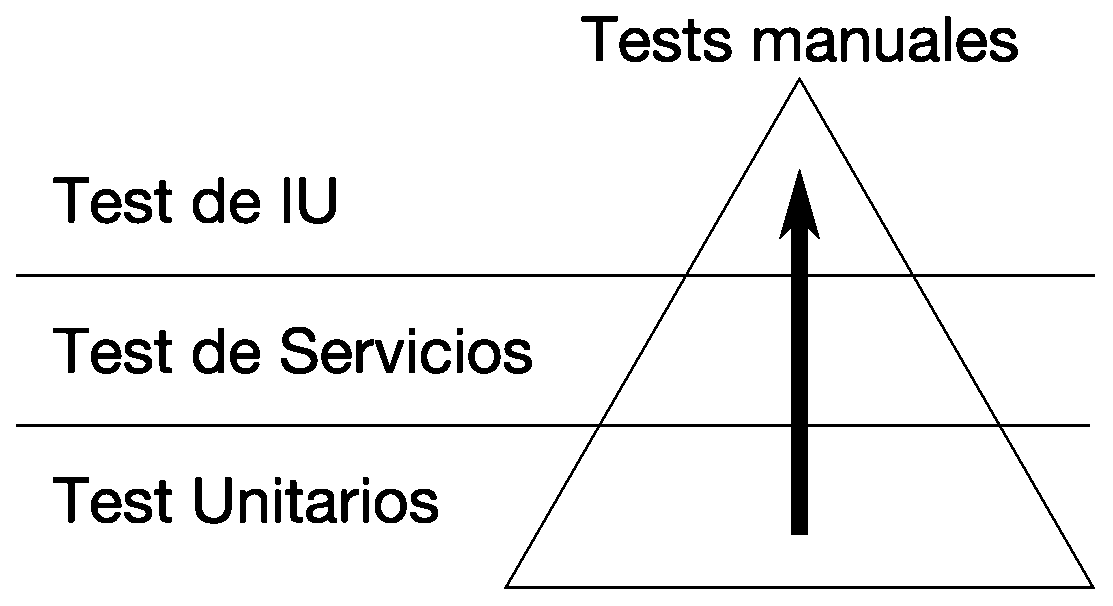
\includegraphics[width=0.5\textwidth]{graphics/pyramid.eps}
\end{figure}
\end{frame}

\begin{frame}
\frametitle{Capa de interfaz de usuario}
Cuando el foco de la evaluación es la interfaz de usuario, se requiere que la
mayoría del código y la lógica de negocio este completamente evaluados. El
enfoque se centra en simplemente asegurarse de que la propia interfaz de
usuario este funcionando correctamente.
\end{frame}

\subsection{Criterios de calidad}

\begin{frame}
\frametitle{Criterios de calidad}
Se denomina criterio de calidad a cualquier requerimiento que define lo que el
producto debe ser.

Se definieron los siguientes como criterios de calidad fundamentales para el
éxito del producto:

\begin{itemize}
\item Usabilidad.
\item Confiabilidad.
\item Compatibilidad.
\end{itemize}
\end{frame}

\subsection{Técnicas de prueba}

\begin{frame}
\frametitle{Técnicas de prueba}
\begin{itemize}
\item Pruebas de aceptación.
\item Pruebas funcionales.
\item Pruebas de dominio.
\item Pruebas negativas.
\end{itemize}
\end{frame}

\section{Análisis del Software}

\begin{frame}
\frametitle{Análisis del Software}
\begin{columns}
\column{0.5\textwidth}
\textbf{Módulos de Productos}
\begin{itemize}
\item Enumerar todas las funciones.
\item Enumerar todas las vistas.
\item Enumerar todos los formularios.
\item Análisis de valores limite.
\end{itemize}
\column{0.5\textwidth}
\textbf{Módulos de Productos}
\begin{itemize}
\item Enumerar todas las funciones.
\item Enumerar todas las vistas.
\item Enumerar todos los formularios.
\item Análisis de valores limite.
\end{itemize}
\end{columns}
\end{frame}

\subsection{Análisis de valor limite}

\begin{frame}
\frametitle{Análisis de valor limite}
\tiny
\begin{table}
\centering
\begin{tabular}{|p{2.6cm}|l|l|l|}
\hline
\footnotesize{\textbf{Variable}} & \footnotesize{\textbf{Casos Posibles}} & \footnotesize{\textbf{Casos Inválidos}} & \footnotesize{\textbf{Limites}} \\
\hline
\footnotesize{Nombre del producto} & \footnotesize{[1-255] caracteres} & & \footnotesize{0} \\
& & \footnotesize{0} & \footnotesize{1} \\
& & \footnotesize{$>$255} & \footnotesize{255} \\
& & & \footnotesize{256} \\
\hline
\footnotesize{Activo} & \footnotesize{\{verdadero,falso\}} & & \\
\hline
\footnotesize{Código de producto} & \footnotesize{[0-255] caracteres} & & \footnotesize{0} \\
& & \footnotesize{$>$255} & \footnotesize{255} \\
& & & \footnotesize{256} \\
\hline
\footnotesize{Familia de productos} & \footnotesize{ninguno,[lista de valores]} & & \\
\hline
\footnotesize{Programación de cantidades activada} & \footnotesize{\{verdadero,falso\}} & & \\
\hline
\footnotesize{Programación de ingresos activada} & \footnotesize{\{verdadero,falso\}} & & \\
\hline
\footnotesize{Descripción del producto} & \footnotesize{[0,4000] caracteres} & & \footnotesize{0} \\
& & \footnotesize{$>$4000} & \footnotesize{4000} \\
& & & \footnotesize{4001} \\
\hline
\end{tabular}
\end{table}
\end{frame}

\section{Casos de Prueba}

\begin{frame}
\frametitle{Casos de Prueba según el tipo de evaluación realizada.}
\begin{figure}
\centering
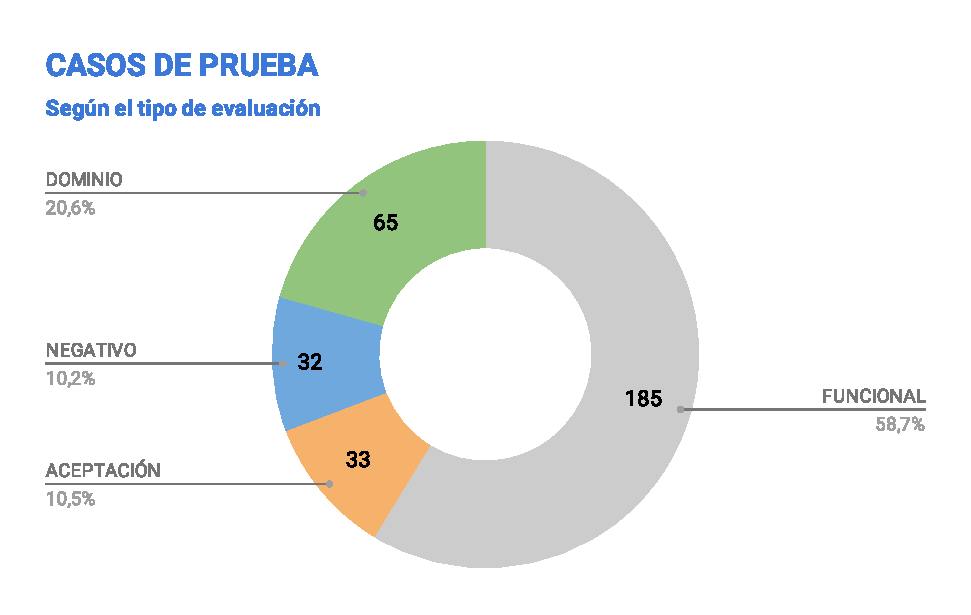
\includegraphics[width=1.0\textwidth]{graphics/tc-tests.eps}
\end{figure}
\end{frame}

\begin{frame}
\frametitle{Casos de Prueba según el tipo de acción a evaluar.}
\begin{figure}
\centering
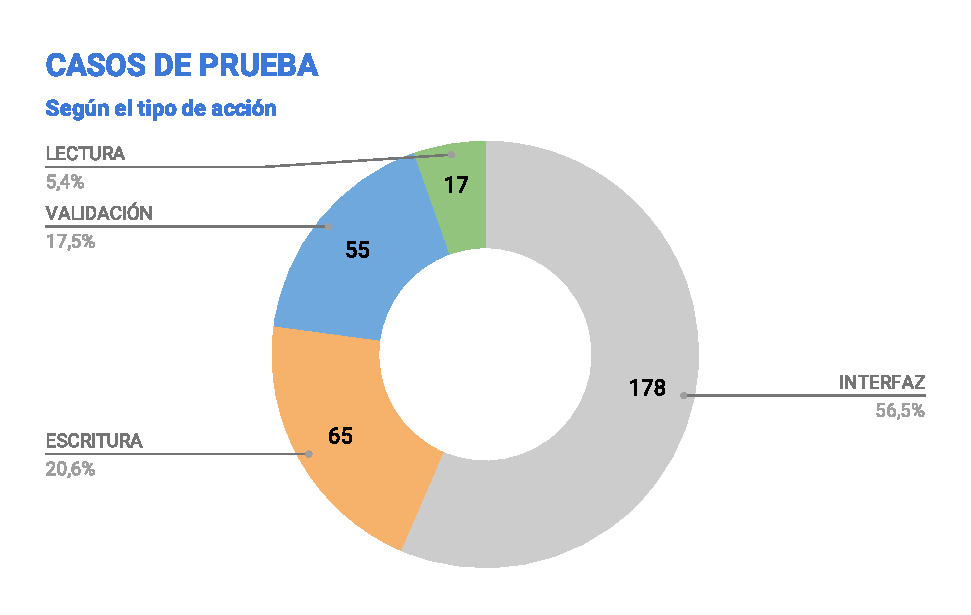
\includegraphics[width=1.0\textwidth]{graphics/tc-type.eps}
\end{figure}
\end{frame}

\section{Desarrollo del framework}

\begin{frame}
\frametitle{Page Object}
\emph{Page Object} sirve para mejorar el mantenimiento de las pruebas y reducir
la duplicación del código.

Un \emph{Page Object} es una clase orientada a
objetos que sirve como la representación de los elementos de una pagina del
software a evaluar.

Las pruebas utilizan los métodos de esta clase cuando
necesitan interactuar con la interfaz de usuario de la pagina a la que hace
referencia.

El beneficio es que si la interfaz de usuario de la pagina cambia,
las pruebas en sí no necesitan cambiar, solo el código dentro del
\emph{Page Object} necesitará actualizarse.
\end{frame}

\begin{frame}
\frametitle{Diagrama de clases sobre las relaciones entre \emph{Page Objects}.}
\begin{figure}
\centering
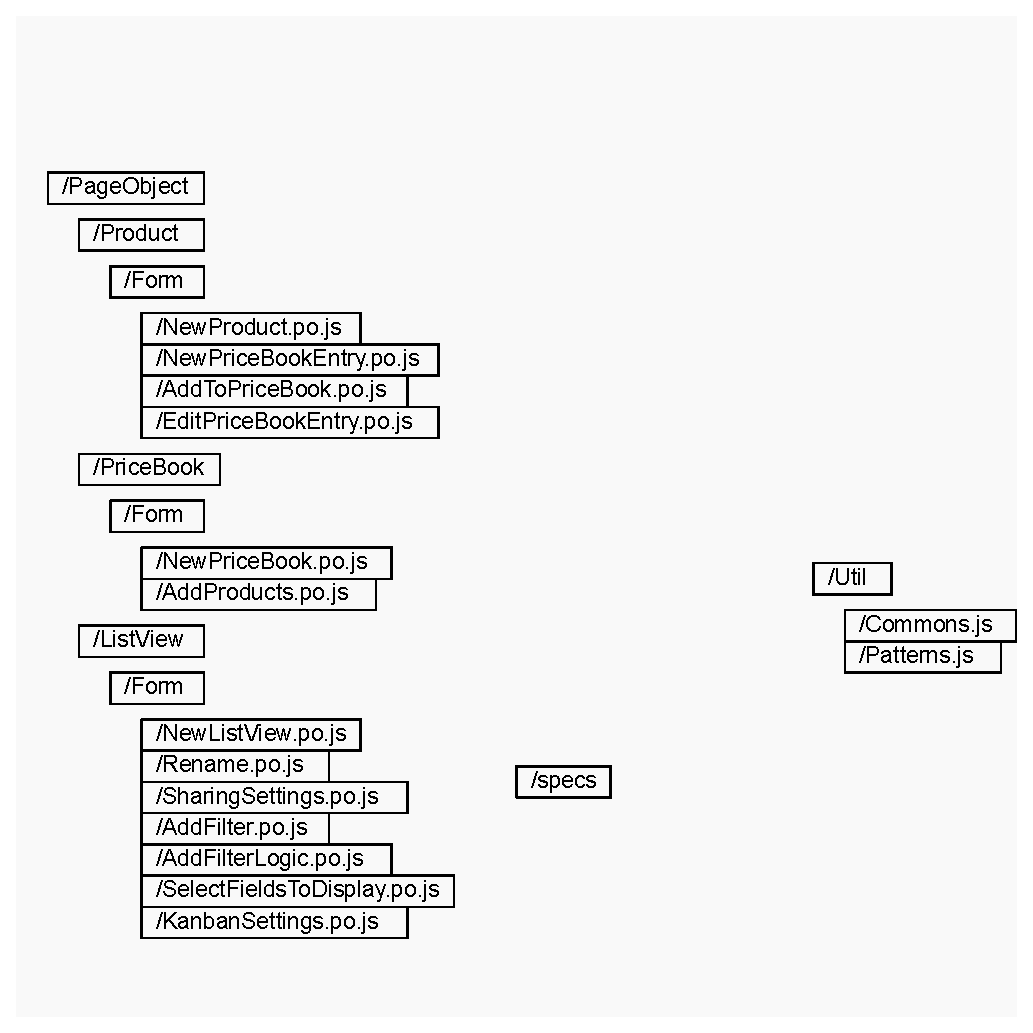
\includegraphics[width=0.8\textwidth]{graphics/diagram01.eps}
\end{figure}
\end{frame}

\begin{frame}
\frametitle{Diagrama de secuencia para el Caso de Prueba A001.}
\begin{figure}
\centering
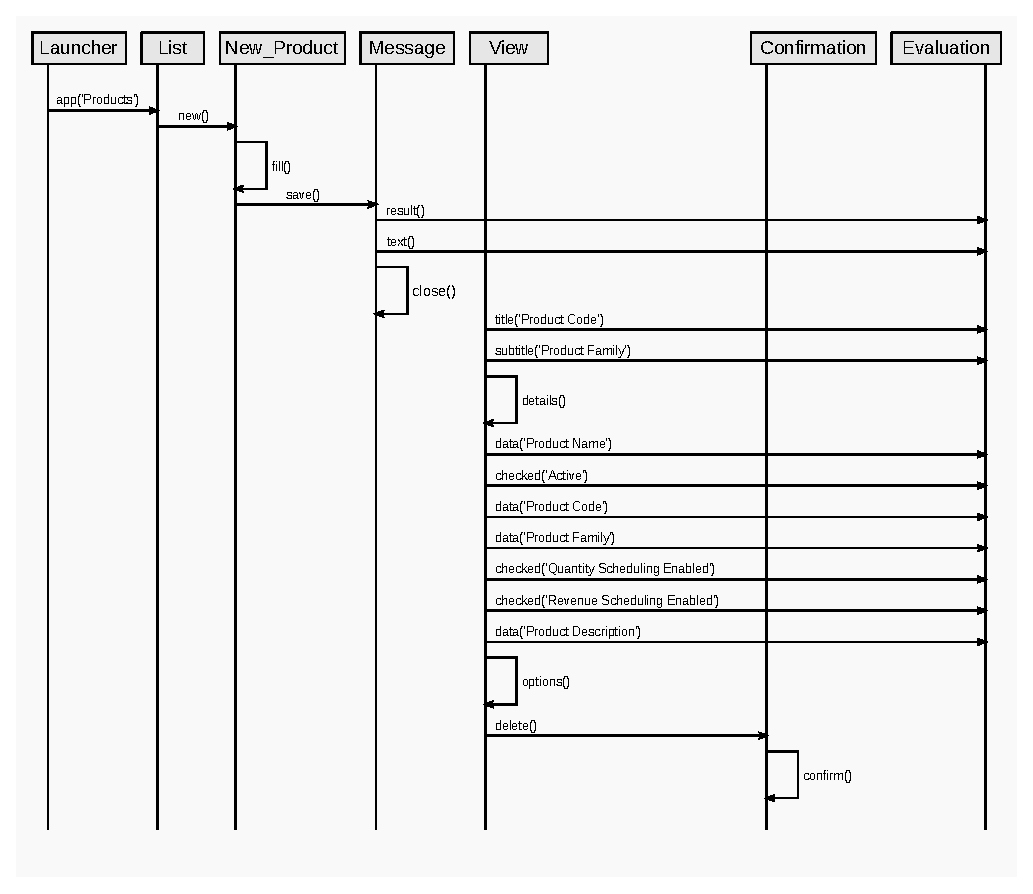
\includegraphics[width=0.8\textwidth]{graphics/diagram02.eps}
\end{figure}
\end{frame}

\begin{frame}
\frametitle{Resultados de las pruebas clasificadas por tipo de evaluación.}
\begin{figure}
\centering
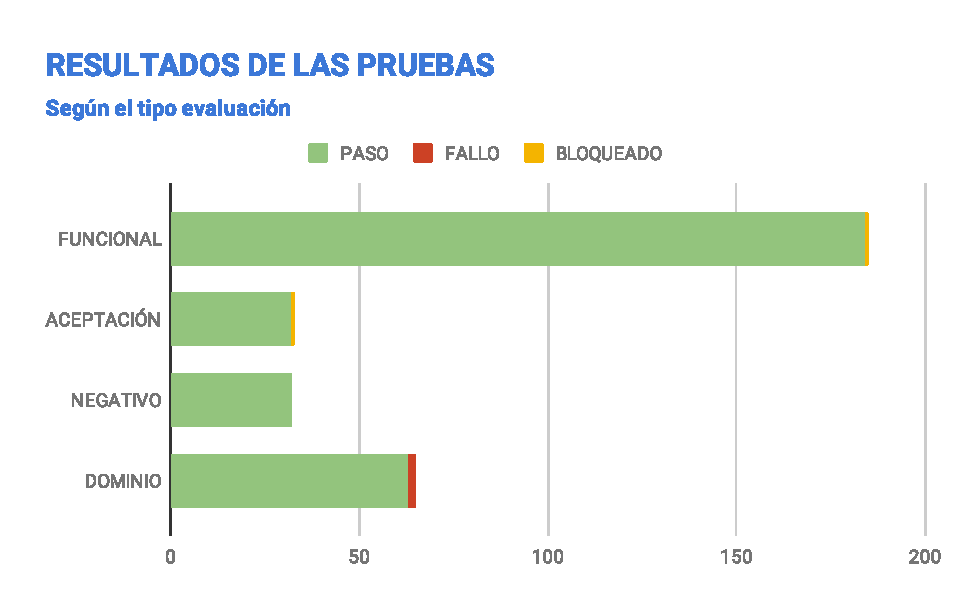
\includegraphics[width=1.0\textwidth]{graphics/results-tests.eps}
\end{figure}
\end{frame}

\begin{frame}
\frametitle{Resultados de las pruebas clasificadas por tipo de acción a evaluar.}
\begin{figure}
\centering
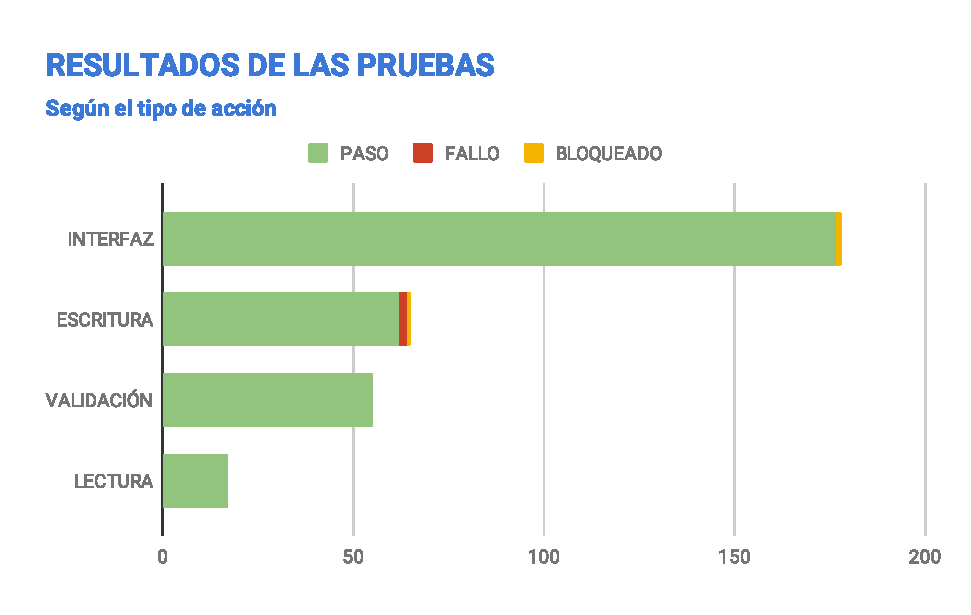
\includegraphics[width=1.0\textwidth]{graphics/results-type.eps}
\end{figure}
\end{frame}

\begin{frame}
\frametitle{Casos de prueba que resultaron no exitosos.}
\begin{table}
\tiny
\centering
\begin{tabular}{|c|p{5.4cm}|c|c|c|}
\hline
\footnotesize{\textbf{Código}} & \footnotesize{\textbf{Caso de Prueba}} &
\footnotesize{\textbf{Resultado}} \\
\hline
\footnotesize{\emph{A007}} &
\footnotesize{Precio de producto para una lista de precios es registrado después
de accionado el botón «Guardar»} &
\footnotesize{Bloqueado} 
\\
\footnotesize{\emph{F041}} &
\footnotesize{Mensaje «Se guardó Entrada del catálogo de precios ."» se muestra
después de modificado un precio} &
\footnotesize{Bloqueado}
\\
\footnotesize{\emph{D017}} &
\footnotesize{Formulario «Agregar a lista de precios» permite el registro,
cuando en el campo «Lista de precios» se ingresa el valor Nulo} &
\footnotesize{Fallido} 
\\
\footnotesize{\emph{D018}} &
\footnotesize{Formulario «Agregar a lista de precios» permite el registro,
cuando en el campo «Divisa» se ingresa el valor Nulo} &
\footnotesize{Fallido}
\\
\hline
\end{tabular}
\end{table}

\end{frame}

\end{document}

